\section{Comparing wave flux divergence to source term area integral}\label{appendix:flux-vs-area}

To the authors knowledge the source term method for computing the local wave resource is being introduced in this work for the first time. Since the source term method cannot be validated directly, it will be compared against the results obtained from the energy flux method under idealized conditions. The local resource using the energy flux method under idealized conditions is computed by subtracting the wave energy flux exiting the domain from that entering the domain using Equation~\eqref{eqn:RR}. In the absence of sources and sinks of energy other than wind input, dissipation due to whitecapping, and quadruple interactions, the difference between the incoming and outgoing energy flux reveals the local resource.

WW3 is implemented in an idealized model over a bathymetry with a constant depth of 4 km covering a region that is 240$^{\circ}$ in the zonal direction and 60$^{\circ}$ in the meridional direction as shown in Figure~\ref{fig:idealizedDomain}a. Deep water was selected to remove the effects of energy convergence or divergence by refraction, and shallow water effects such as depth-induced wave breaking and bottom friction. We consider a hypothetical EEZ as a proxy for a region of interest. Energy flux is computed at 200 nautical miles from the eastern end of the domain, which we approximate in the model as 3$^{\circ}$20’ from the eastern boundary given the model domain has been centered at the Equator. This hypothetical EEZ covers 20$^{\circ}$ in the meridional direction as shown in Figure~\ref{fig:idealizedDomain}a. The area of this region is 818,000 km$^{2}$, which is comparable in size to the US West Coast EEZ (825,550 km$^{2}$). In the meridional direction the model spatial resolution is a constant 1$^{\circ}$ (111.12 km), while in the zonal direction the spatial resolution is reduced from 1$^{\circ}$ (111.12 km at the Equator) to 4’ (7.4 km) close to the EEZ (see Figure~\ref{fig:idealizedDomain}b) to be consistent with the models used in the hindcast.
 
\begin{figure}[ht]
  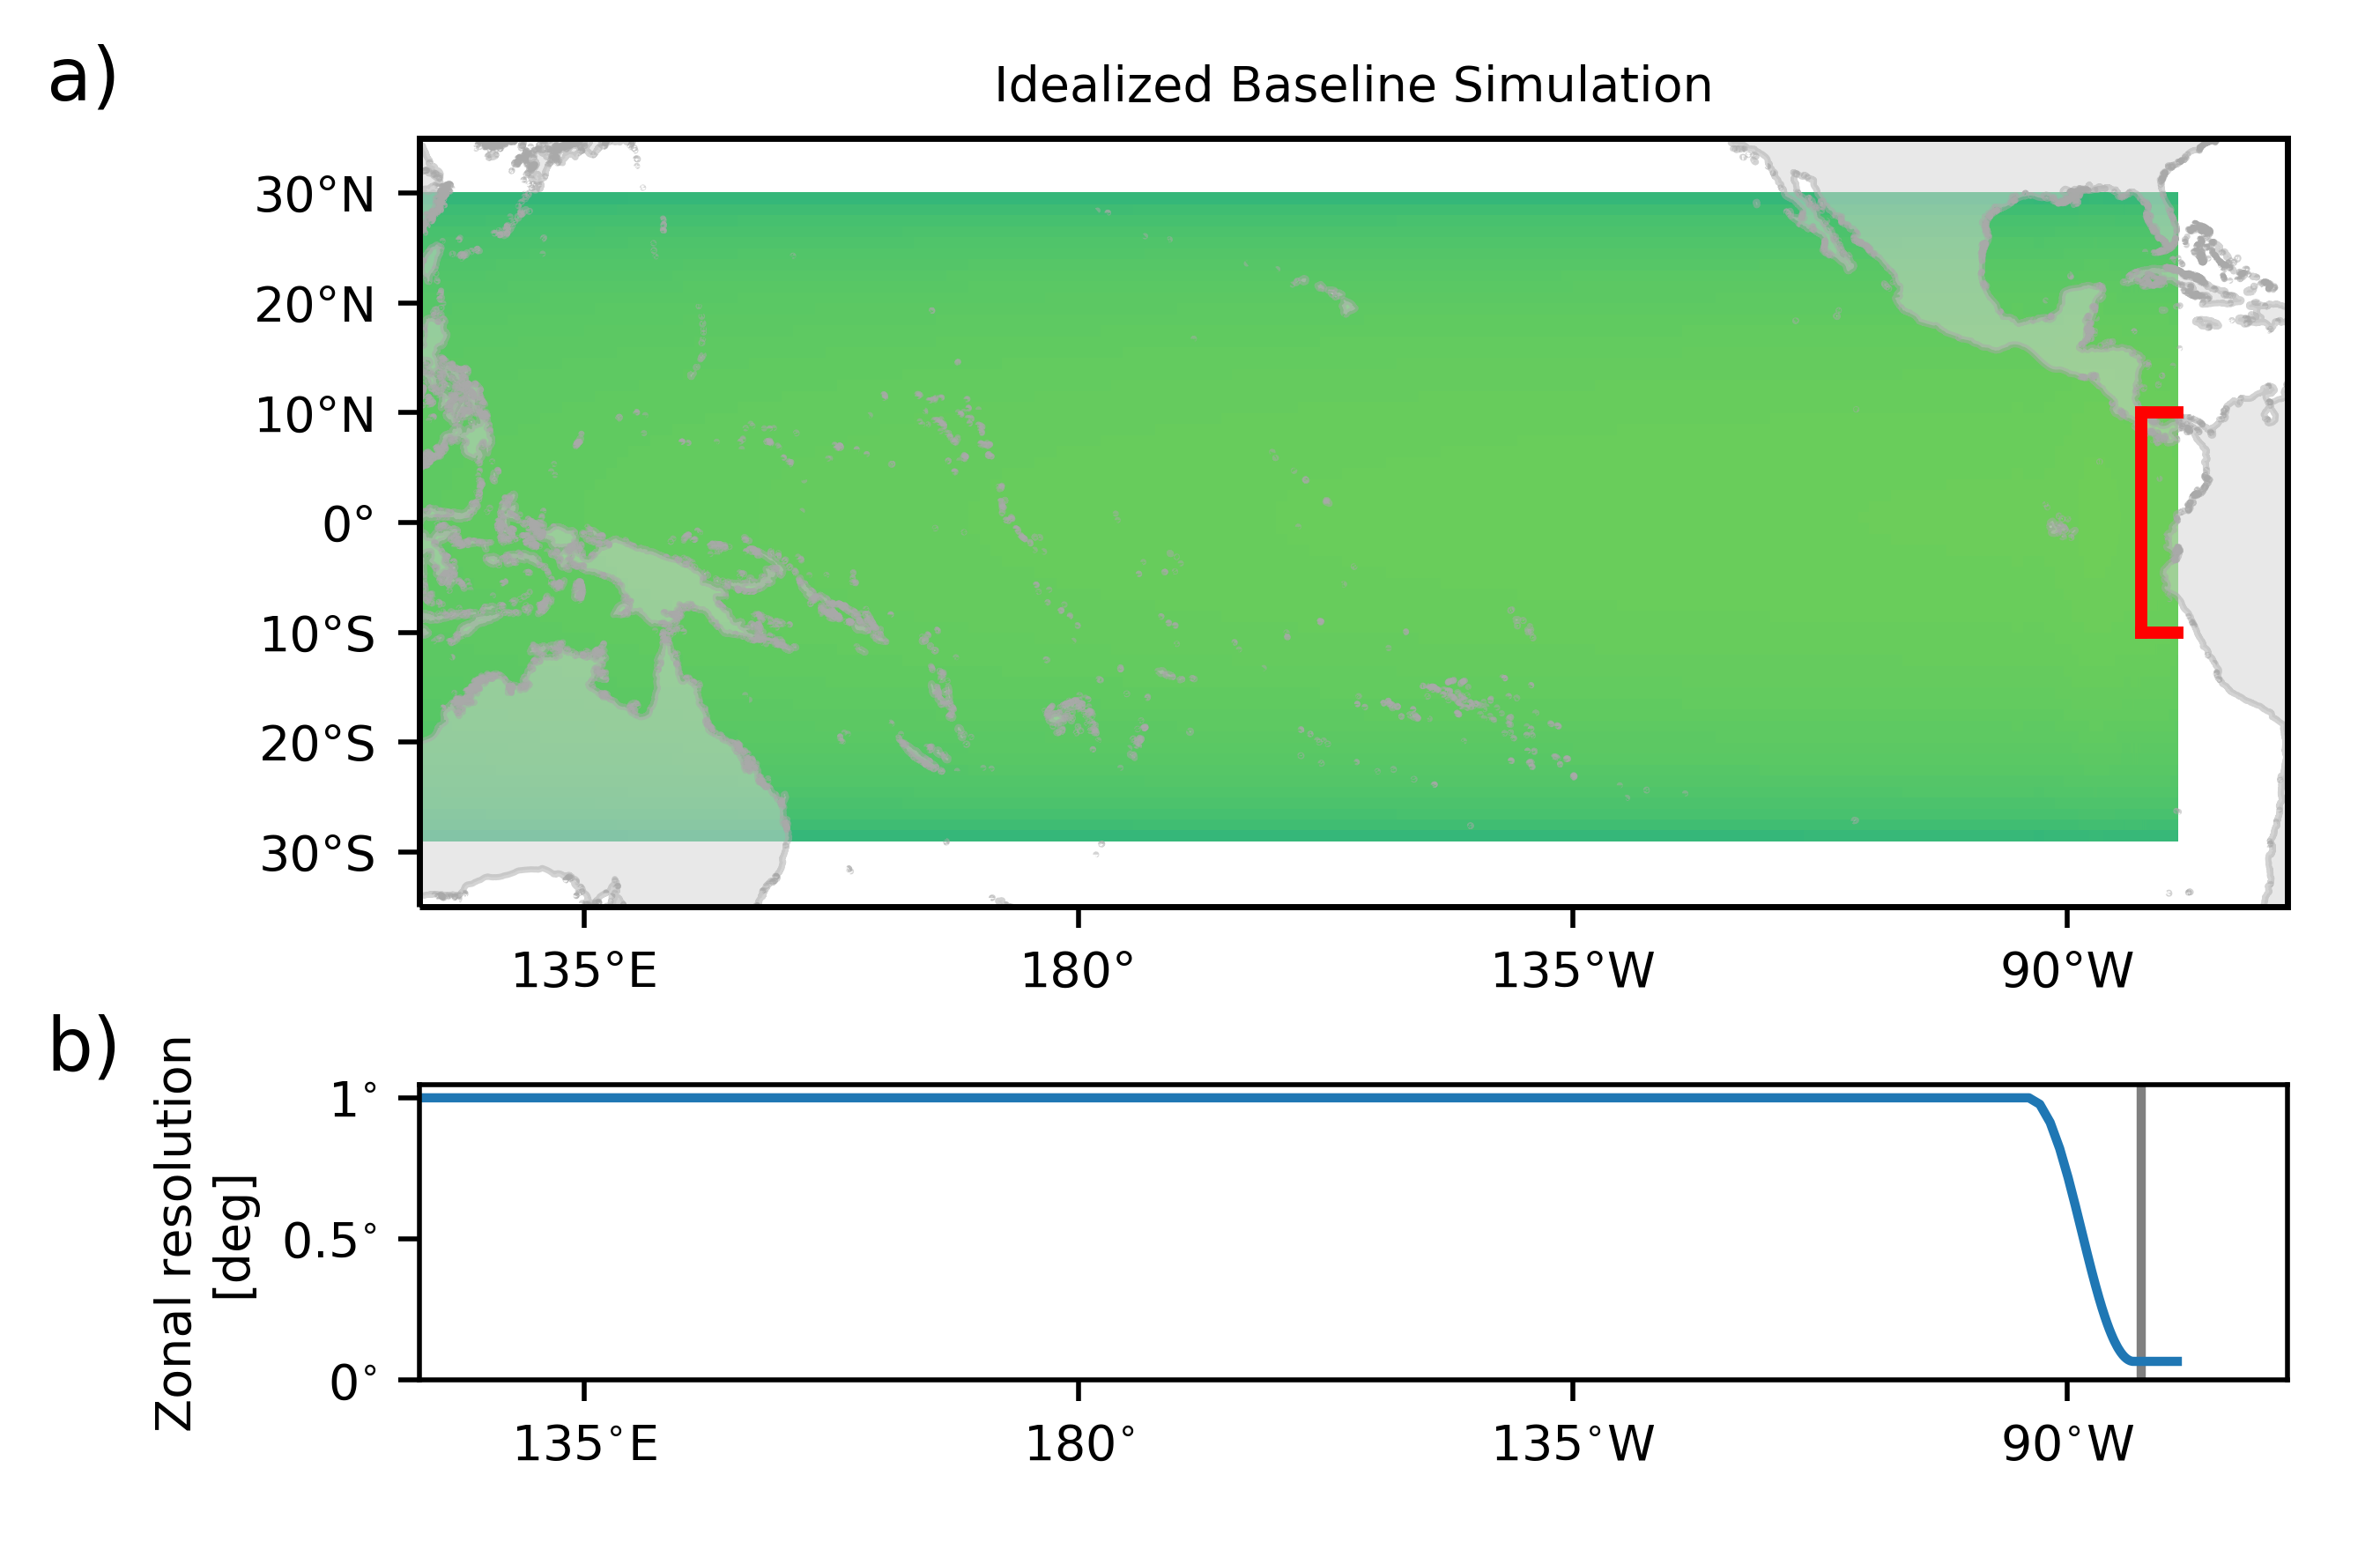
\includegraphics[width=4.5in]{../../diagram/appendixB_Figure1.png}
  \caption{a) Idealized model grid with the analysis zone identified with a red box. Continents are added for visualizing the scale of the model only, the model domain is a basin with constant depth. b) Zonal resolution of the model grid.}
  \label{fig:idealizedDomain}
\end{figure}

For all the idealized simulations, a stationary 7.0 m/s westerly wind is applied over the entire domain. The wind speed is based on the yearly averaged wind speed measured at NDBC stations 46005 and 46002 offshore the U.S. West Coast (\url{https://www.ndbc.noaa.gov/}), which are 7.3 and 7.0 m/s, respectively. The model domain was selected to be long enough such that the waves achieve energy equilibrium (i.e., constant wave height and period) west of the analysis zone. The model is executed for three months, where the results from the first two months are discarded to ensure steady state. The two methods of computing the local resource, energy flux and source term, are compared by analyzing two different scenarios of the idealized model. For both scenarios, the model is forced by a constant westerly wind west of the EEZ but only one of them has local wind forcing east of the EEZ. Wave energy flux collected at the end of the simulation period along the Equator is shown in Figure~\ref{fig:idealizedOWP}. The results are consistent west of the EEZ where the wind is active in both cases. The remote resource is computed along this line and is very similar for both scenarios as shown in Table~\ref{table:idealizedResource}. There is a decrease of wave power just westward of the EEZ (where the wind stops acting), which is attributed to the northern and southern model open boundaries having upstream effects on the wave field.

\begin{figure}[ht]
  \centering
  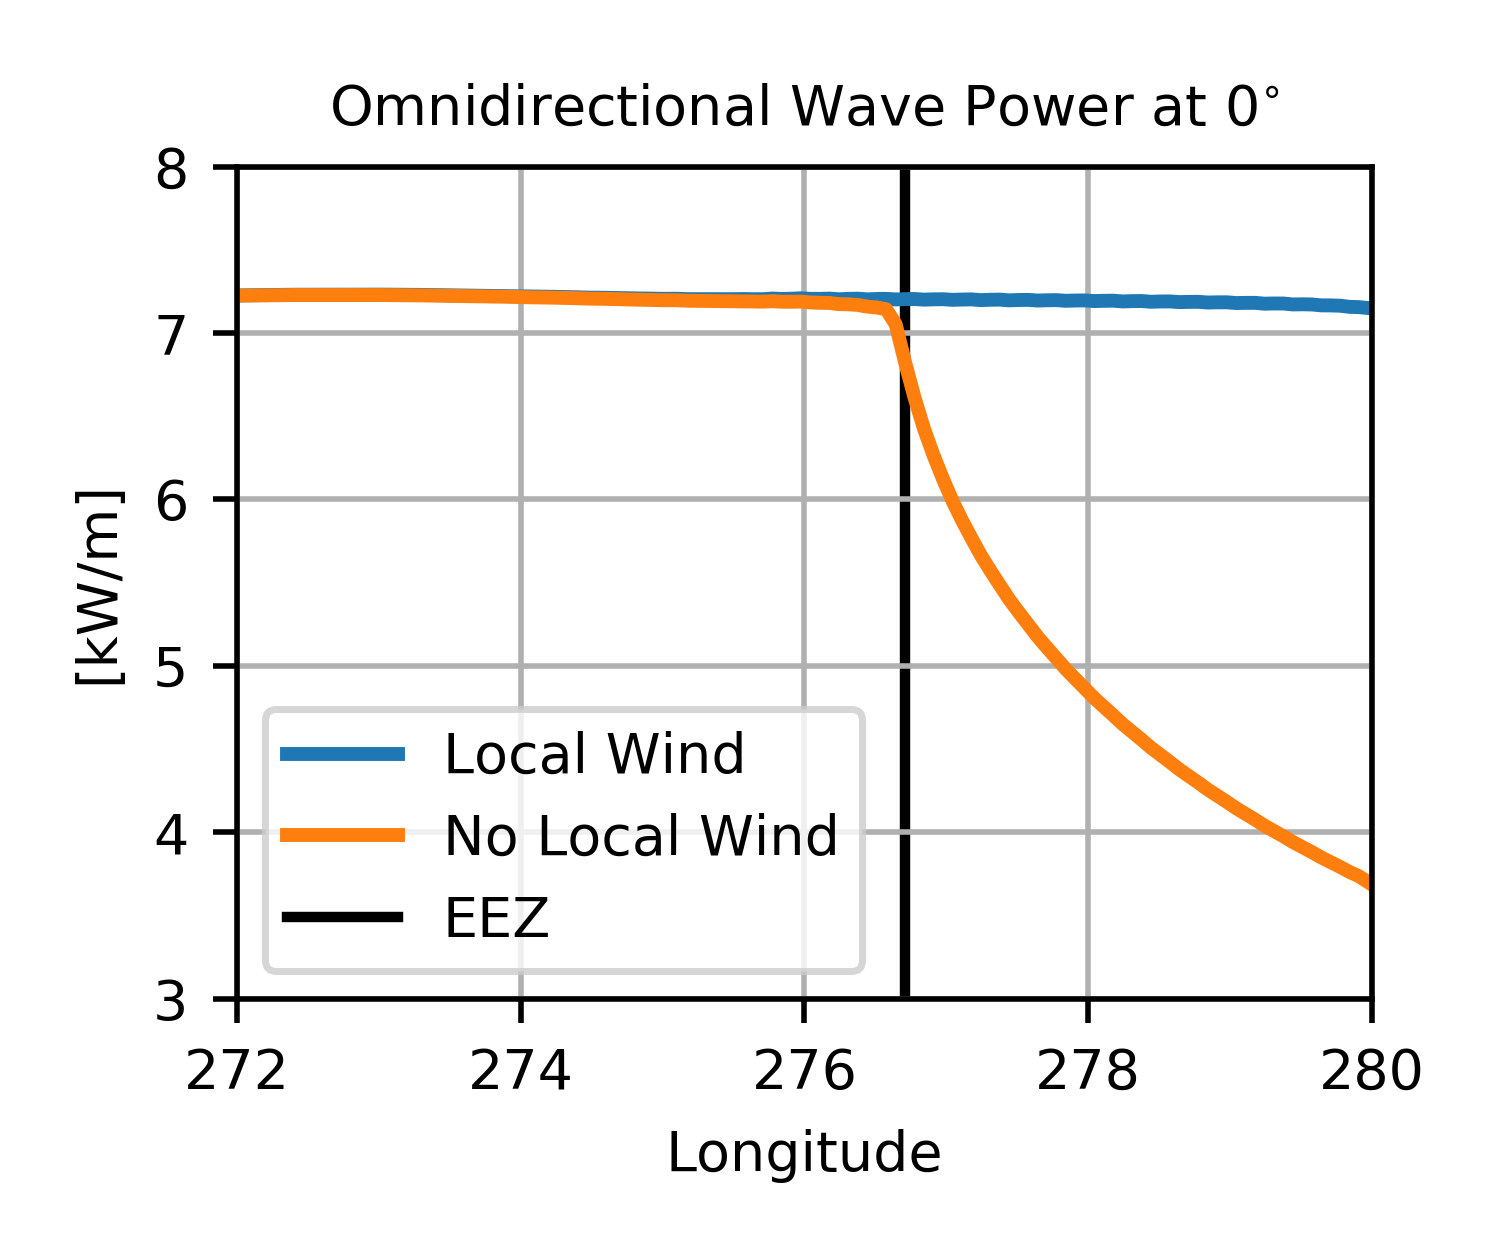
\includegraphics[width=3in]{../../diagram/appendixB_Figure2.png}
  \caption{Wave energy flux across the middle of the domain with and without local wind forcing.}
  \label{fig:idealizedOWP}
\end{figure}

In the case of no local wind the wave power starts decreasing quickly eastward of the EEZ. This is because of the swell dissipation component of $S_{in}$ source term \citep{ardhuinObservationSwellDissipation2009}. The total dissipation rate decreases eastward due to the propagation of the swell in this direction. The local resource for such a scenario is negative. It is worth noting that the contribution of $S_{ds}$ to the total balance is zero because there is no active wave growth that would be balanced by whitecapping. The local wave energy resource from both approaches yield similar results as shown in Table~\ref{table:idealizedResource}. In this example the loss of wave energy amounts to 37\% of the remote resource. 

On the other hand, when the waves have reached a stead state (known as a fully developed sea), the local wave resource is, by definition, zero. Computing the local resource from both approaches yield results very close to zero as well (Table~\ref{table:idealizedResource}). For this condition the wave energy flux is constant with longitude (as observed from Figure~\ref{fig:idealizedOWP}) and, based on our definition, computing the energy flux across different meridians and subtracting them will result in zero local resource. In this case swell dissipation is countered by wind wave growth at high frequencies which is then transferred to the lower frequencies via the non-linear interactions.

\begin{table}[ht]
  \centering
  \begin{tabular}{cccc}
    \hline
    Local Wind & Remote Resource & Local Resource: Energy Flux & Local Resource: Source Terms \\
    \hline
    No  & 12.94 & -5.44 & -5.49 \\
    Yes & 13.42 & -0.02 &  0.15 \\
\hline
  \end{tabular}
  \caption{Wave energy resource for idealized basin in GW}
  \label{table:idealizedResource}
\end{table}

Both approaches produce very similar results given that the waves have an eastward travel direction, thus avoiding the shortcomings of the energy flux method discussed in Section~\ref{sec:method}. Therefore, the source term method is suitable to estimate the local resource.
